\documentclass[12pt]{article}

\usepackage{config/sbc-template}
\usepackage{float}
\usepackage{graphicx,url}
\usepackage{comment}
\usepackage[brazil]{babel}   
%\usepackage[latin1]{inputenc}  
\usepackage[utf8]{inputenc}  
% UTF-8 encoding is recommended by ShareLaTex
\usepackage{listings}

\renewcommand{\lstlistingname}{Código}

\lstset{ %
  aboveskip=10px, % space between the list frame and normal text
  %backgroundcolor=\color{white},   % choose the background color; you must add \usepackage{color} or \usepackage{xcolor}
  basicstyle=\small,                 % the size of the fonts that are used for the code
  xleftmargin=15px,
  belowskip=20px, % space that text will appear after listing frame
  breakatwhitespace=true,         % sets if automatic breaks should only happen at whitespace
  breaklines=true,                 % sets automatic line breaking
  captionpos=b,                    % sets the caption-position to bottom
  commentstyle=\color{mygreen},    % comment style
  %deletekeywords={},            % if you want to delete keywords from the given language
  %escapeinside={\%*}{*)},          % if you want to add LaTeX within your code
  extendedchars=true,              % lets you use non-ASCII characters; for 8-bits encodings only, does not work with UTF-8
  frame=single,                    % adds a frame around the code
  keepspaces=true,                 % keeps spaces in text, useful for keeping indentation of code (possibly needs columns=flexible)
  %keywordstyle=\color{blue},       % keyword style
  language=R,                 % the language of the code
  %otherkeywords={},           % if you want to add more keywords to the set
  numbers=left,                    % where to put the line-numbers; possible values are (none, left, right)
  numbersep=5pt,                   % how far the line-numbers are from the code
  %numberstyle=\tiny\color{mygray}, % the style that is used for the line-numbers
  %rulecolor=\color{black},         % if not set, the frame-color may be changed on line-breaks within not-black text (e.g. comments (green here))
  showspaces=false,                % show spaces everywhere adding particular underscores; it overrides 'showstringspaces'
  showstringspaces=false,          % underline spaces within strings only
  %showtabs=false,                  % show tabs within strings adding particular underscores
  stepnumber=1,                    % the step between two line-numbers. If it's 1, each line will be numbered
  %stringstyle=\color{mymauve},     % string literal style
  tabsize=2,                       % sets default tabsize to 2 spaces
  %title=\lstname                   % show the filename of files included with %\lstinputlisting; also try caption instead of title
}
     
\sloppy

\title{Projeto de Simulação no NS-3 (Rede sem Fio)}

\author{Felipe Lima Morais\inst{1}, Diogo Machado Gonçalves\inst{1},}


\address{Instituto de Computação -- Universidade Estadual de Campinas
  (UNICAMP)\\
  Campinas -- SP -- Brasil
  \email{felipelimamorais@gmail.com, diogomachadogoncalves@gmail.com}
}

\begin{document} 

\maketitle

\begin{resumo} 
Como parte da avaliação da disciplina de MO655 - Gerência de Redes do programa de Pós graduação em Ciência da Computação do Instituto de Computação da Unicamp, este relatório apresenta os passos executados na construção de uma simulação de rede sem fio utilizando o simulador NS-3. A simulação consiste na avaliação de dispositivos que se comunicação através de uma rede sem fio, enviando pacotes para um servidor ligado ao ponto de acesso (AP) sem fio, utilizando modelos de tráfego em rajada e CBR. Para avaliar variados cenários, redes formadas exclusivamente por nós móveis e nós estáticos foram construídas, além de avaliar o desempenho dos modelos de tráfego por rajada e CBR nessas redes. Resultados mostraram, através das métricas vazão, perda de pacotes e tempo de atraso na entrega de pacotes, que redes realizando tráfego em rajada apresentaram um volume de pacotes perdidos e uma vazão inferiores às redes configuradas somente com nós utilizando CBR. A utilização de nós móveis afetou pouco o desempenho dos nós utilizando CBR, porém, para tráfego em rajada houve uma decréscimo de desempenho nas redes avaliadas.
\end{resumo}

\section{Introdução}

Este relatório técnico apresenta as configurações utilizadas para a implementação de duas situações simuladas, sendo a situação onde os nós possuem mobilidade e a outra onde eles não possuem a mobilidade. Descrevendo também as funções e os parâmetros utilizados para gerar as variações no tipo de tráfego de dados da redes, que poder ser rajada ou (CBR - \textit{Constante Bit Rate}).

Essas simulações foram feitas no simulador NS-3 na versão 3.26. O código que realiza as simulações foi desenvolvido em C++ e as informações coletadas, foram armazenadas em arquivos (csv -\textit{Comma-separated values}), que possibilitaram o desenvolvimento de gráficos utilizando a linguagem R. 

Este relatório descreve as alterações que uma rede sem fio pode sofrer a medida que se aumenta a quantidade de nós, proporcionando uma analise comparativa entre os tipos de tráfegos, juntamente com a variação do tipo de mobilidades implementada nos nós. 

O restante deste relatório está organizado da seguinte forma: A seção~\ref{projeto} descreve detalhadamente como é cada cenários desenvolvido. Já a seção~\ref{dev} apresenta como foi desenvolvido as simulações no NS-3 utilizando C++ e também como foi gerado os   \textit{scripts} e os gráficos usando a linguagem em R. Na seção~\ref{sec::resultados} apresentamos as analises realizadas, junto dos gráficos gerados, e as conclusões estarão presentes na seção~\ref{sec::resultados}



\section{Projeto e Critérios de Implementação}
\label{projeto} \label{sec:proj_e_criterios}

O projeto a ser executado consiste na simulação de uma Rede sem Fio 802.11 no modo infraestruturado com um Ponto de Acesso realizando a interconexão entre todos os dispositivos móveis a um servidor conectado ao ponto de acesso através uma conexão ponto a ponto. A simulação desta rede será realizada utilizado o simulador de redes baseado em eventos discretos NS-3. O simulador NS-3 \cite{henderson2008network, riley2010ns} possui uma versão estável desde 2008 e atualmente está na versão ns-3.26.

A execução do projeto divide-se na simulação de duas situações envolvendo a rede sem fio descrita. Em um primeiro experimento considera-se uma rede com dispositivos de acesso sem fio sem mobilidade. As métricas utilizadas para medir o desempenho desses dispositivos posicionados ao redor do ponto de acesso se dará por meio da vazão de dados enviados, atraso no recebimento de pacote e a taxa de pacotes perdidos na transmissão.

O espaço em que os dispositivos estão alocados é de 100 metros quadrados, sendo posicionados de uma forma uniformemente aleatória. O ponto de acesso, em todas as simulações, é definido no centro desse espaço (posição x=50 e y=50).

No primeiro experimento, as métricas serão coletadas a partir do ponto de vista da rede como um todo, além de apresentar os dados dos dispositivos mais próximo e mais distante ao ponto de acesso. A fim de permitir uma comparação com a visão dos nós mais distante e mais perto do pronto de acesso, os resultados para a rede como um todo serão e apresentados como a média dentre todos os dispositivos atuantes na simulação, incluindo os dois dispositivos enquadrados nos casos especiais anteriormente descritos.
    
Em um segundo experimento, repete-se a abordagem do primeiro experimento mas agora considera-se também a mobilidade dos dispositivos de comunicação sem fio. O simulador NS-3 oferece diversos modelos para a simulação da mobilidade dos nós. Para a execução deste trabalho foi utilizada a função ns3::GaussMarkovMobilityModel para a mobilidade, configurada para realizar movimentos em uma velocidade de 2 à 7 km/hora em variadas direções. Neste experimento não será avaliado o desempenho dos nós mais distante e mais próximo ao ponto de acesso.

A comunicação entre os dispositivos e o ponto de acesso é realizada utilizando dois modelos de tráfego, um utilizando uma taxa constante de transmissão CBR e outro realizando tráfego em rajada. A variação no protocolo de comunicação é avaliada em todos os cenários descritos anteriormente.

Para o modelo de tráfego em rajada, o protocolo utilizado na comunicação é o TCP, em que cada pacote enviado possui 1500 bytes. Para o tráfego CBR o protocolo utilizado é o UDP com pacotes de 512 bytes. A implementação desses modelos de tráfego foi realizada utilizando uma aplicação do tipo \textit{OnOff} que realiza o envio de pacotes alternando entre períodos de envio e períodos de espera. Para tráfego em rajada alterna entre 2 segundo de envio de pacotes para cada 3 segundos de espera. Para tráfego constante a aplicação alterna entre 1 milissegundo de envio e um milissegundo de espera. Em ambos os modelos de tráfego o canal de comunicação entre os dispositivos e o ponto de acesso possui um \textit{data rate} de 512 kbps.

Considerando os experimentos 1 e 2, onde existe critérios de avaliação apresentados nas 4 cenários, sendo eles, o protocolo TCP sem mobilidade, o protocolo TCP com mobilidade, o protocolo UPD sem mobilidade e o protocolo UPD com mobilidade. Em cada uma dessas combinações as métricas de avaliação relativas a vazão, atraso e perda de pacotes deverá ser avaliada.

A captura desses dados é feita através de um modulo disponível no NS-3 chamado \textit{Flow monitor}. Este módulo oferece métodos para avaliar uma conexão baseada nas métricas exigidas, vazão, atraso, e perda de pacotes. O monitoramento de cada conexão tem como saída a média dos dados gerados pela métrica escolhida de acordo com o tempo em que a conexão se manteve ativa.

Para avaliar a escalabilidade da rede e as consequências de um crescimento no número de dispositivos conectados ao ponto de acesso, os cenários apresentados foram submetidos a testes considerando o número de dispositivos dentro do conjunto 5, 10, 15, 20, 25, 30, 35 e 40.

A fim de validar os resultados obtidos para cada um dos cenários propostos, os resultados serão apresentados seguindo um intervalo de confiança de 95$\%$. Para cada uma das médias apresentadas, uma taxa de erro que será associada ao objetivo de indicar que há 95$\%$ de probabilidade da média de experimentos reais estarem contida naquele intervalo.

Quanto maior o conjunto de dados que compõem a média desses experimentos, maior a confiabilidade das médias apresentadas e por consequência, menor a taxa de erro a ser considerada para enquadrar o intervalo de confiança de 95$\%$. Para computar a média foram realizadas 30 execuções de cada um dos cenários apresentados, em que cada execução tinha a duração de 60 segundos. A média dessas execuções são apresentadas nos gráficos da seção \ref{sec::resultados}, junto com seus respectivas taxas de erro calculadas para o intervalo de confiança de 95$\%$.

\section{Desenvolvimento}
\label{dev}

O código necessário para a implementação da simulação no NS-3 de todos os cenários descritos no projeto divide-se basicamente em 3 arquivos: \textit{script\_de\_execucao.R}, \textit{script\_de\_graficos.R} e \textit{wifi\_infra.cc}. O último é uma implementação feita em C++ que realiza a simulação em sí. Os dois primeiros são \textit{scripts} implementados na linguarem R para execução da simulação, fornecendo os devidos parâmetros para a execução de \textit{wifi\_infra.cc}, além de gerar e validar os resultados.

Destalhes de implementação de cada arquivo são descritos com mais detalhes nas subseções seguintes.

\subsection{Script de execução}

O \textit{script} \textit{script\_de\_execucao.R} é o responsável por execução automática de todo o conjunto de teste. O Código \ref{alg:script_de_execucao} basicamente executa um laço de repetição variando o número dispositivos que irão atuar na simulação (de 5 à 40, aumentando de 5 em 5 a cada iteração). O sistema configura as variáveis para a escolha da semente que gerará os números pseudo-aleatórios utilizados pelo código \textit{wifi\_infra.cc}, dentre eles a definição da posição dos dispositivos.

A cada iteração, os 4 cenários da simulação são executados, tráfego CBR em nós estáticos, tráfego CBR em nós móveis, tráfego em rajada em nós estáticos e tráfego em rajada em nós móveis. A execução de cada cenário está configurada para durar 60 segundos e o resultado de cada execução gera um arquivo (CSV - Comma-separated Values) com a média dos resultados para cada um dos critérios.

\begin{lstlisting}[language=R, caption=Laço de repetição aplicado na execução da simulação, label=alg:script_de_execucao]
for (i in seq(from=5, to=40, by=5)){
  rand <- sample(1:9382, 1)
  print("CBR e nos fixos")
  system(paste("NS_GLOBAL_VALUE=\"RngRun=", rand,"\" ./waf --run \"scratch/wifiinfra --nodes=",i," --runningTime=60 --traffic=true --mobility=false --printLog=false --prefix=\\\"",args[1],"\\\"   \"", collapse=", ", sep=""))
  print("CBR e nos moveis") #CBR e nos fixos
  system(paste("NS_GLOBAL_VALUE=\"RngRun=", rand,"\" ./waf --run \"scratch/wifiinfra --nodes=",i," --runningTime=60 --traffic=true --mobility=true --printLog=false --prefix=\\\"",args[1],"\\\"    \"", collapse=", ", sep=""))
  print("Rajada e nos fixos")
  system(paste("NS_GLOBAL_VALUE=\"RngRun=", rand,"\" ./waf --run \"scratch/wifiinfra --nodes=",i," --runningTime=60 --traffic=false --mobility=false --printLog=false --prefix=\\\"",args[1],"\\\"   \"", collapse=", ", sep=""))
  print("Rajada e nos moveis")
  system(paste("NS_GLOBAL_VALUE=\"RngRun=", rand,"\" ./waf --run \"scratch/wifiinfra --nodes=",i," --runningTime=60 --traffic=false --mobility=true --printLog=false --prefix=\\\"",args[1],"\\\"   \"", collapse=", ", sep=""))
}
\end{lstlisting}

\subsection{Script para geração dos resultados}

O \textit{script} \textit{script\_de\_graficos.R} é o responsável por coordenar e processar os dados gerados por cada execução da simulação. O \textit{script} realiza, como apresentado no Código \ref{alg:call_repeticoes}, o controle do número de execuções que um mesmo cenário será executado a fim de se gerar a média desse conjunto. O número de repetições é passada por parâmetro para o \textit{script}. Neste trabalho foi definida a geração da média a partir de 30 execuções de cada cenário. A cada iteração o \textit{script\_de\_execucao.R} é executado, gerando os arquivos CSV correspondentes.

Após cada chamada ao \textit{script\_de\_execucao.R}, os dados salvos nos arquivos CSV são lidos e salvos em uma respectiva matriz cubica de acordo com a métrica utilizada na execução. Ao total são geradas 8 matrizes, para o primeiro experimento: cube\_cp\_cbr (CBR/Nós estáticos), cube\_cp\_pulse (Rajada/Nós estáticos), cube\_n\_cbr (CBR/Nó mais próximo), cube\_n\_pulse (Rajada/Nó mais próximo), cube\_f\_cbr (CBR/Nó mais distante) e cube\_f\_pulse (Rajada/Nó mais distante), e para o segundo experimento: cube\_rw\_cbr (CBR/Nós móveis) e cube\_rw\_pulse (Rajada/Nós móveis).

Os índices 2 à $n$+1 do eixo $z$ recebem os valores gerados por cada uma das $n$ execuções da simulação. O primeiro índice no eixo $z$ de cada matriz recebe a média das demais índices. O cálculo é realizado pela função \textit{calc\_result (matriz)}, como ilustrado no Código \ref{alg:calc_resultados}.

Cada coluna da matriz contém os dados de uma métrica (Vazão, atraso e perda) e cada linha indica o número de dispositivos presentes na execução da simulação.

\begin{lstlisting}[language=R, caption=Laço de repetição para execução da simulação, label=alg:call_repeticoes]
for (i in args[2]:args[1]){
  if (args[3]){
    print(paste("Execute ", i, sep=" "))
    system(paste("Rscript script_de_execucao.R", i, sep=" "))
  }
\end{lstlisting}

\begin{lstlisting}[language=R, caption=Geração dos resultados, label=alg:calc_resultados]
calc_result <- function(cube){

  for (i in 1:nrow(cube) ){
    for (j in 1:ncol(cube)) {
      cube[i,j,1] <- mean(cube[i,j,2:(as.integer(args[1])+1)])
    }
  }
  return (cube)
}

cube_rw_cbr <- calc_result(cube_rw_cbr)
cube_cp_cbr <- calc_result(cube_cp_cbr)
cube_rw_pulse <- calc_result(cube_rw_pulse)
cube_cp_pulse <- calc_result(cube_cp_pulse)
cube_n_cbr <- calc_result(cube_n_cbr)
cube_n_pulse <- calc_result(cube_n_pulse)
cube_f_cbr <- calc_result(cube_f_cbr)
cube_f_pulse <- calc_result(cube_f_pulse)

\end{lstlisting}

Após a leitura de todos os dados gerados, o cálculo da taxa de erro para o intervalo de confiança é calculado para cada ponto a ser inserido no gráfico. O cálculo é realizado pela função \textit{calc\_error(matriz)}, apresentado no Código \ref{alg:taxa_de_erro_ic}, no qual seque a fórmula (coeficiente de confiança) * (desvio padrão do conjunto)/($\sqrt(n)$), onde o coeficiente de confiança é obtido na tabela de distribuição normal com base no intervalo de confiança de 95$\%$ e $n$ sendo o número de execuções de cada cenário, no caso 30.

Após todos os cálculos, por fim os respectivos gráficos são gerados a partir dos resultados presentes nas matrizes.

\begin{lstlisting}[language=R, caption=Cálculo da taxa de erro para o intervalo de confiança, label=alg:taxa_de_erro_ic]
calc_error <- function(matrix){
  result <- array(dim=c(nrow(matrix)))
  for(i in 1:nrow(matrix)){
    n <- length(matrix[i,2:(as.integer(args[1])+1)])
    sd <- sd(matrix[i,2:(as.integer(args[1])+1)])
    coef_de_conf <- 1.96
    result[i] <- (coef_de_conf) * (sd/sqrt(n))
  }
  return(result)
}
\end{lstlisting}


\subsection{Código CPP para simulação no NS-3}

O código \textit{wifi\_infra.cc} é o principal código dentre os 3 arquivos e a implementação da simulação em si.

A rede sem fio utilizada é composta por $n$ dispositivos conectados a um ponto de acesso através de comunicação sem fio. Conectado ao ponto de acesso também se encontra uma conexão ponto a ponto ligando o ponto de acesso a um servidor. A simulação consiste no envio de pacotes dos dispositivos para o servidor intermediado pelo ponto de acesso.

O fluxo de execução da simulação é dada pela função run() apresentada no Código \ref{alg:wifi_run}. Inicialmente são declarados os nós dos dispositivos, do ponto de acesso e dos nós ligados pela conexão ponto a ponto, seguidos pelas declaração das interfaces de rede de cada \textit{device} e suas respectivas interfaces para atribuição de IPs.

As linhas 7 à 9 instanciam o número de nós referentes aos seus respectivos tipos. O nó relacionado ao ponto de acesso é o mesmo que linha uma das pontas do canal ponto a ponto. O número de dispositivos instanciados está relacionado a variável \textit{nNodes} atribuída por parâmetro na execução do código \textit{wifi\_infra.cc}.

A função \textit{setMobility()} (linha 11) é chamada para atribuição dos parâmetros de mobilidade dos dispositivos. O ponto de acesso possui uma localização fixa em todas os cenários. Sua localização é estática na posição (50,50) do ambiente. Os dispositivos são distribuídos aleatoriamente seguindo uma distribuição uniforme em uma área de 100 metros quadrados. A mobilidade desses dispositivos depende do parâmetro passado para o algoritmo durante sua chamada de execução. Caso o usuário deseje que os nós sejam móveis, a variável \textit{mobility} será atribuída com o  valor booleano verdadeiro e os dispositivos terão um padrão de mobilidade seguindo o modelo \textit{Gauss Markov}, caso contrário seguirão estáticos nas posições definidas. A cada execução do algoritmo a posição inicial dos nós é alterada.

Após a definição do modelo de mobilidade dos dispositivos, a função \textit{installP2PDevices()} (linha 13) é chamada para definir a taxa de transmissão do canal ponto a ponto que conecta o ponto de acesso ao servidor. A taxa de transmissão escolhida foi 5 Mbps.

A função \textit{installWirelessp2pdevice()}  instancia as camadas \textit{mac} e \textit{phy} nos dispositivos e no ponto de acesso. Em seguida a função \textit{installInternetProtocol()} instala uma camada TCP/IP e atribui os IPs para o ponto de acesso e para os dispositivos. A função \textit{PopulateRoutingTables()} (linha 20) é chamada para preencher as tabelas de roteamentos dos nós da rede.

O condicional da linha 23 verifica qual modelo de tráfego de dados será utilizado. A variável \textit{traffic} é atribuída de acordo com o parâmetro recebido na execução do código \textit{wifi\_infra.cc}. Caso o valor da variável seja verdadeira o tráfego a ser utilizado é CBR utilizando o protocolo UDP, senão o tráfego será em Rajada e o protocolo utilizado será TCP.

A função \textit{installUDPCommunication()} define o protocolo UDP na comunicação entre os dispositivos e o ponto de acesso e realiza a instanciação da aplicação \textit{OnOff} para transmitir os pacotes de 512 bytes em um canal de 512 kbps, entre os dispositivos e o ponto de acesso. Cada dispositivos se conecta à uma porta do servidor. A aplicação está configurada para alternar entre 1 ms enviando dados e 1 ms inativa.

A função \textit{installTCPCommunication()} exerce o mesmo papel da função anterior, porém aplicando o protocolo TCP em um tráfego em rajada. Os pacotes nesse modelo possuem 1500 bytes e são enviados em um canal de 512 kbps. A aplicação está configurada para enviar dados alternadamente por 2 segundos e esperar por 3 segundos.

Em seguida, o maneira escolhida para monitorar o tráfego da rede foi utilizando o módulo \textit{Flow monitor}, disponível no simulador. As linhas 29 e 30 declaram uma instancia do módulo e configuram o monitoramento para todos os nós da rede.

As linhas 33 e 34 definem o momento de encerrar a execução da simulação. A variável \textit{runningTime} é atribuída de acordo com o parâmetro recebido na execução de \textit{wifi\_infra.cc}. Para a geração da base de teste o tempo de execução da aplicação foi definido com 60 segundos. Foi acrescido 1 segundo como o tempo para a inicialização da aplicação e 1 segundo como tempo para a simulação se encerrar após o termino de execução da aplicação.

A linha 37 gera um arquivo \textit{xml} com os dados da rede monitorados pelo \textit{Flow monitor} mas para a geração dos gráficos os dados utilizados têm origem da função \textit{buildStatistics()}. A função \textit{buildStatistics()} é responsável por filtrar todos os dados capturados pelo \textit{Flow monitor} durante a execução da simulação.

A função calcula, para cada dispositivo da rede, a sua vazão, atraso de pacotes e sua taxa de perda de pacotes. Os dados referentes a vazão são salvos seguindo a média por segundo dos valores gerados e utilizando kbps como base.

Os dados relacionados ao atraso dos pacotes são salvos na relação tempo de atraso por pacote, sendo os dados representados em milissegundos. Os pacotes perdidos são salvos levando em consideração o total durante toda a simulação.

Os dois dispositivos enquadrados nos casos especiais, dispositivo mais perto e mais longe do ponto de acesso, são salvos individualmente nos dois arquivos CSV correspondentes. Os dados gerados por esses dispositivos, além de todos os dados gerados pelos demais irão compor a média daquela simulação, sendo esta média salva em outro arquivo CSV.

De acordo o uso ou não de mobilidade dos dispositivos e de qual modelo de tráfego utilizado, também é de responsabilidade da função \textit{buildStatistics()} salvar as médias dos dados da redes em arquivos CSV próprios. Cada arquivo CSV gerado segue a ordem: número de dispositivos utilizados na simulação, vazão média da rede, atraso médio de pacotes e média de pacotes perdidos por cada dispositivo.

\begin{lstlisting}[language=C++, caption=Função responsável pelo fluxo de execução da simulação, label=alg:wifi_run]
void run (){
  NodeContainer apnode, nodes, p2pnode;
  NetDeviceContainer apdevice, devices, p2pdevice;
  Ipv4InterfaceContainer apdeviceIP, devicesIP, p2pdeviceIP;

  //Create nodes
  p2pnode.Create (2);
  apnode = p2pnode.Get(1);
  nodes.Create (nNodes);

  setMobility(apnode, nodes);

  installP2PDevices(p2pnode, p2pdevice);

  installWirelesp2pdevice(apnode, nodes, apdevice, devices);

  installInternetProtocol(apnode, nodes, p2pnode, apdevice, devices, p2pdevice, apdeviceIP, devicesIP, p2pdeviceIP);

  /* Populate routing table */
  Ipv4GlobalRoutingHelper::PopulateRoutingTables ();

  // if udp/cbr
  if(traffic)
    installUDPCommunication(nodes, p2pdeviceIP);
  else
    installTCPCommunication(nodes, p2pnode, p2pdeviceIP);

  // Install FlowMonitor on all nodes
  FlowMonitorHelper flowmon;
  Ptr<FlowMonitor> monitor = flowmon.InstallAll ();

  // Simulation running time
  Simulator::Stop (Seconds (runningTime+2));
  Simulator::Run ();

  // execute magic of the flowmon
  buildStatistics(flowmon, monitor, devicesIP, p2pdeviceIP);

  // Cleanup
  Simulator::Destroy ();
}
\end{lstlisting}


\section{Resultados}\label{sec::resultados}

Os resultados obtidos das simulações são apresentados nas subseções \ref{subsec:atraso}, \ref{subsec:perda} e \ref{subsec:vazao} referentes ao atraso, perda de pacotes e vazão da rede, respectivamente.

Os dados apresentados são resultado de simulações nos cenários propostos anteriormente, utilizando dispositivos estáticos e móveis e considerando os modelos de tráfego em rajada e CBR.

Para cada cenário avaliado, foram realizadas 30 execuções para se extrair a média a ser apresentada nos gráficos. São comparados os resultados de todos os ambientes de simulação, variando o número de dispositivos que compõem a rede, de 5 em 5 em um intervalo de 5 a 40.

Para cada ponto dos gráficos foi incluída a margem de erro associada à ele de acordo com o intervalo de confiança de 95$\%$ em uma média entre 30 amostras.

\subsection{Atraso}\label{subsec:atraso}

Uma das métricas de avaliação dos cenários foi por meio da medida do tempo médio de atraso na entrega dos pacotes enviados pelos dispositivos para o servidor por meio de um ponto de acesso sem fio.

O gráfico ilustrado na Figura \ref{fig:delay_static} apresenta os resultados de cenários que possuem apenas nós estáticos compondo a rede. O gráfico apresenta os dados referentes ao tempo médio no atraso dos pacotes em dois cenários distintos, um considerando o uso do modelo de tráfego em rajada e utilizando o protocolo TCP e outro adotando o tráfego constante de dados (CBR) e o protocolo UDP. Para cada cenário também foi apresentado os resultados associados aos dispositivos mais próximo e mais distante da localização do ponto de acesso.

\begin{figure}[H]
\begin{center}
{%
\setlength{\fboxsep}{2pt}%
\setlength{\fboxrule}{1pt}%
\fbox{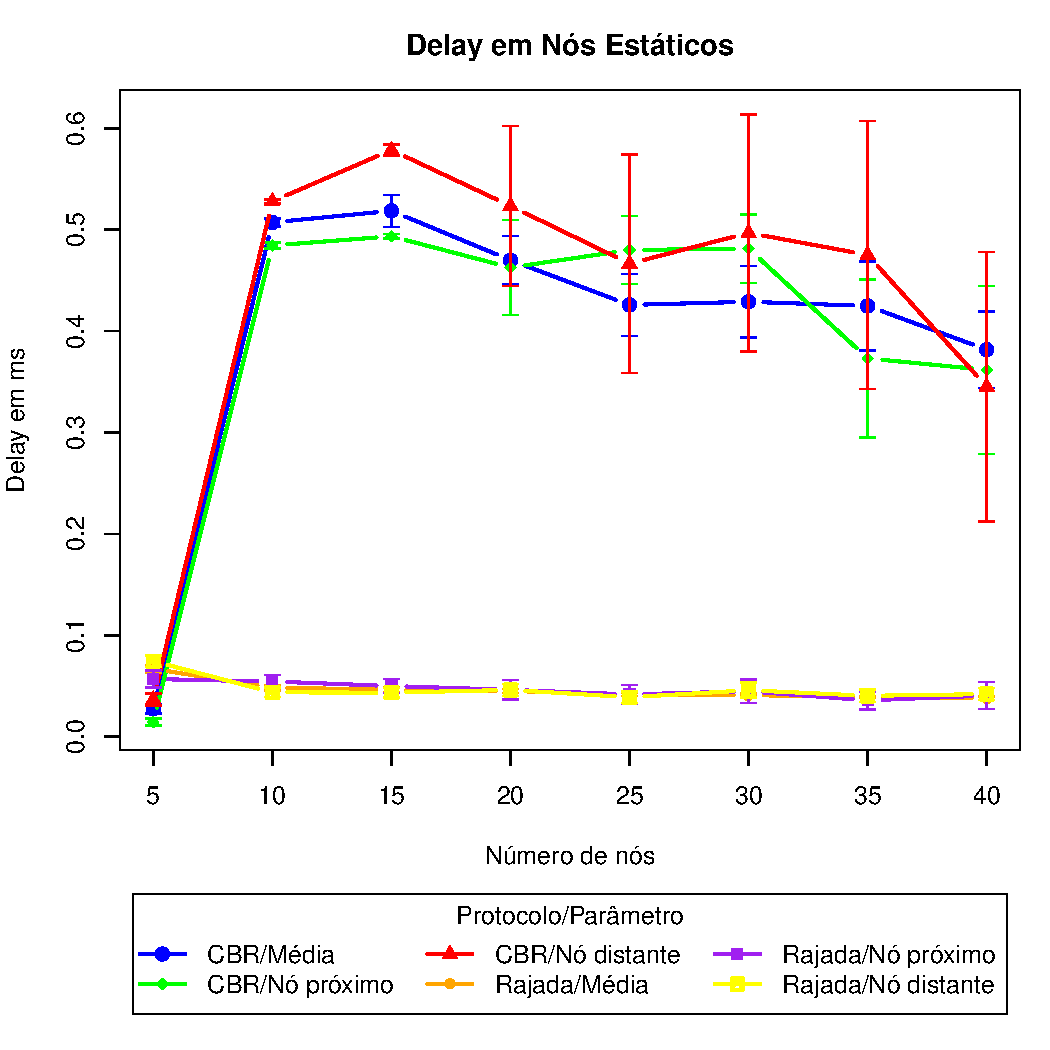
\includegraphics[width=.6\textwidth]{images/Delay_static.pdf}}%
}
\end{center}
\caption{Tempo médio de atraso na entrega dos pacotes a partir de dispositivos sem mobilidade.}
\label{fig:delay_static}
\end{figure}

Para os cenários que adotaram o tráfego CBR, pode-se notar que \textit{delay} superior comparados com os que adotaram o tráfego em rajada. O tráfego CBR apresentou pouca variação de acordo com o aumento no número de dispositivos na rede ao contrário dos cenários que utilizaram tráfego em rajada que apresentaram um grande aumento no tempo de atraso na transição da rede de 5 para 10 dispositivos.

Em geral, os dispositivos mais distantes do ponto de acesso apresentaram um tempo de atraso um pouco superior aos dispositivos mais próximos e à média da rede. As margens de erro associadas aos pontos dos dispositivos mais distantes e mais próximos dos AP se mostraram bem superiores à média devido a geração desses dados ser feita a partir de um conjunto menor de amostras (30) se comparado à média.

Outra maneira de avaliar os resultados apresentados anteriormente é incorporar um modelo de mobilidade por parte dos dispositivos que compõem a rede. A Figura \ref{fig:delay_CBR_pulse} apresenta os resultados referentes ao comportamento da rede ao utilizar os modelos de tráfego em rajada e CBR em ambientes em que os nós possuem mobilidade e em ambientes em que os nós não possuem mobilidade. Os dados apresentados no gráfico ilustram o tempo médio de atraso dos pacotes nesses cenários.

Os cenários que utilizaram uma taxa constante de transferência de dados apresentaram um tempo médio de atraso, a partir de 10 dispositivos, de 4 a 5 vezes superior se comparados com os cenários que adotaram o tráfego em rajada.

Ao se comparar o modelo de mobilidade adotados pelos cenários pode-se notar um aumento pouco significativo no tempo médio de atraso entre as redes que possuem dispositivos com mobilidade comparadas com as redes que possuem dispositivos estáticos.

\begin{figure}[H]
\begin{center}
{%
\setlength{\fboxsep}{2pt}%
\setlength{\fboxrule}{1pt}%
\fbox{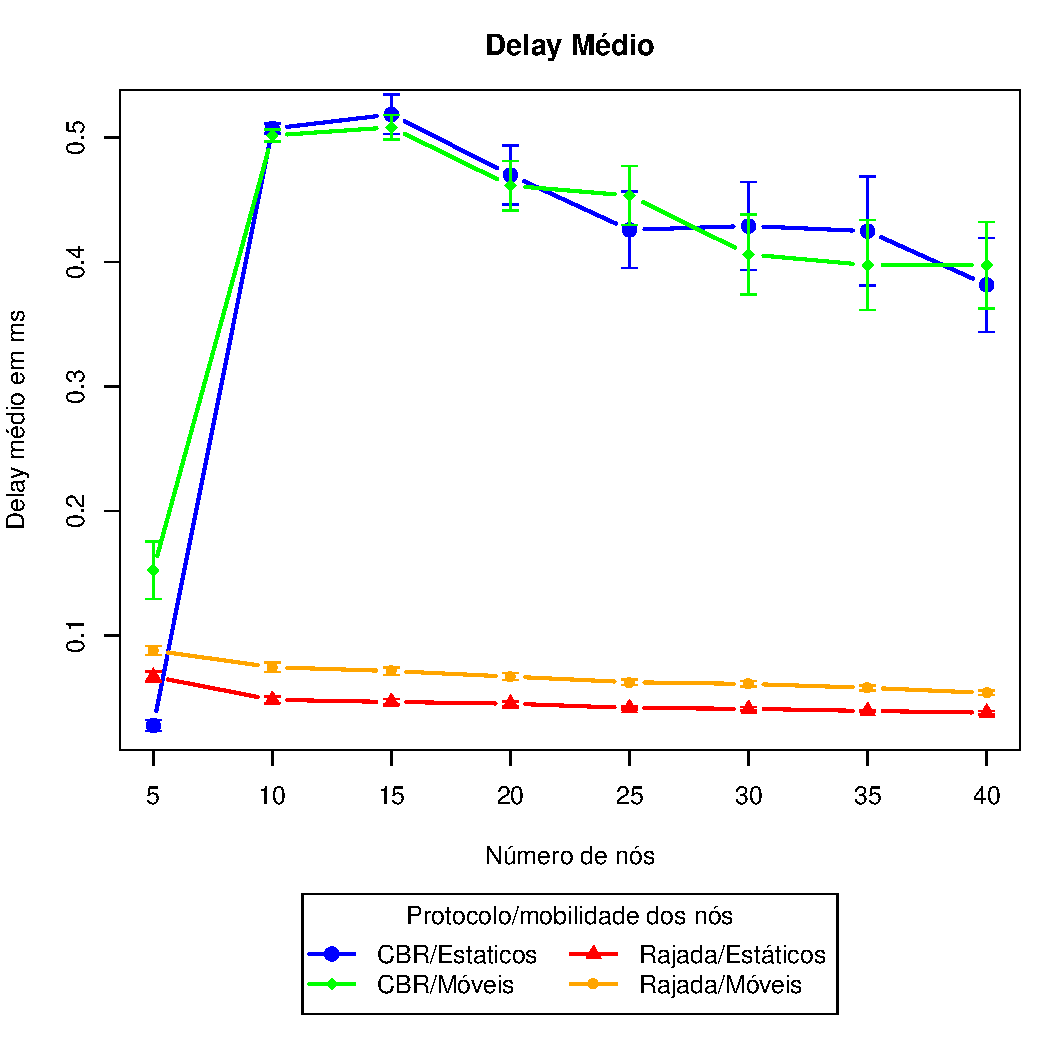
\includegraphics[width=.65\textwidth]{images/Delay_CBR_pulse.pdf}}%
}
\end{center}
\caption{Tempo médio de atraso na entrega dos pacotes na rede.}
\label{fig:delay_CBR_pulse}
\end{figure}

%\begin{figure}[H]
%\begin{center}
%{%
%\setlength{\fboxsep}{2pt}%
%\setlength{\fboxrule}{1pt}%
%\fbox{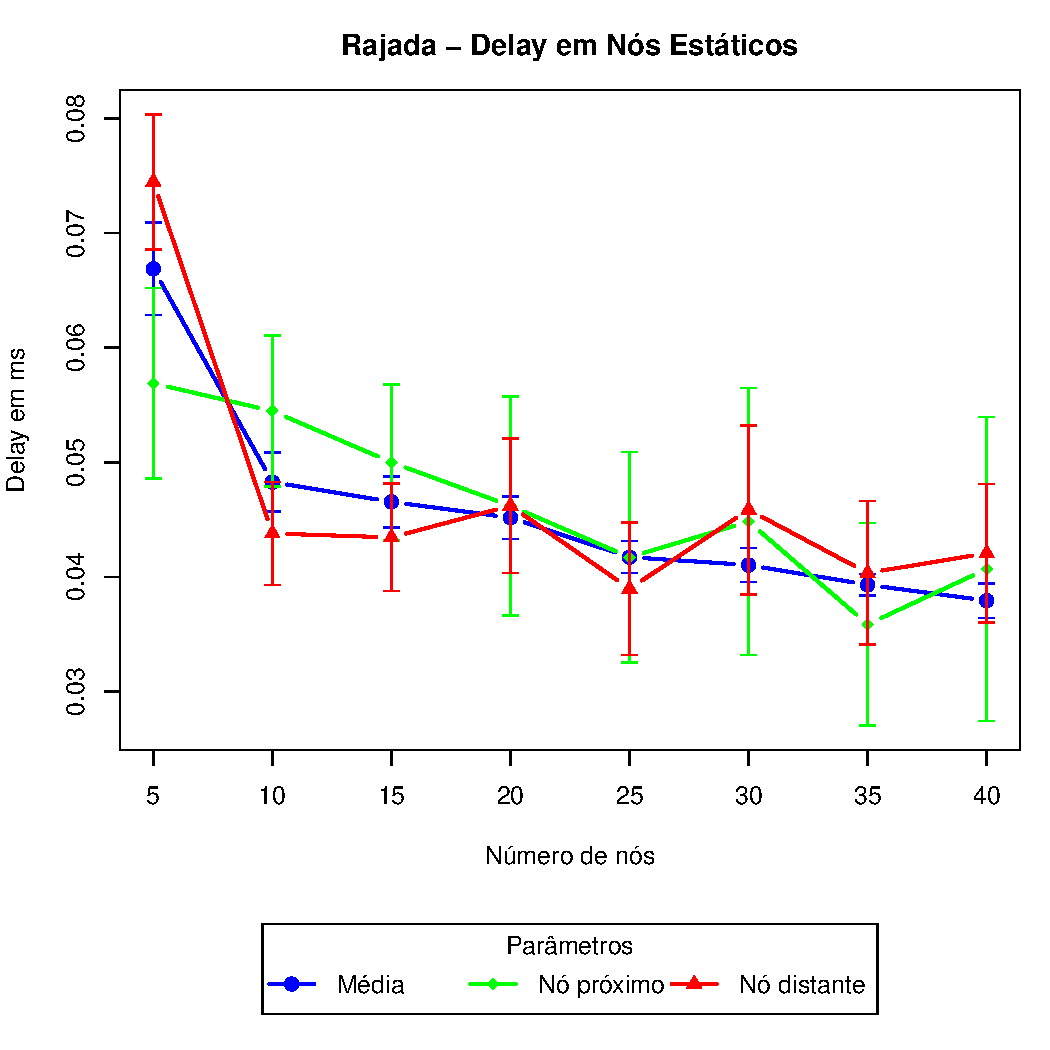
\includegraphics[width=.7\textwidth]{images/DelayPackets_static_pulse.pdf}}%
%}
%\end{center}
%\caption{Tempo médio de atraso na entrega de pacotes a partir de nós sem mobilidade utilizando tráfego em rajada (Rajada/TCP).}
%\label{fig:delayPackets_static_pulse}
%\end{figure}

%\begin{figure}[H]
%\begin{center}
%{%
%\setlength{\fboxsep}{2pt}%
%\setlength{\fboxrule}{1pt}%
%\fbox{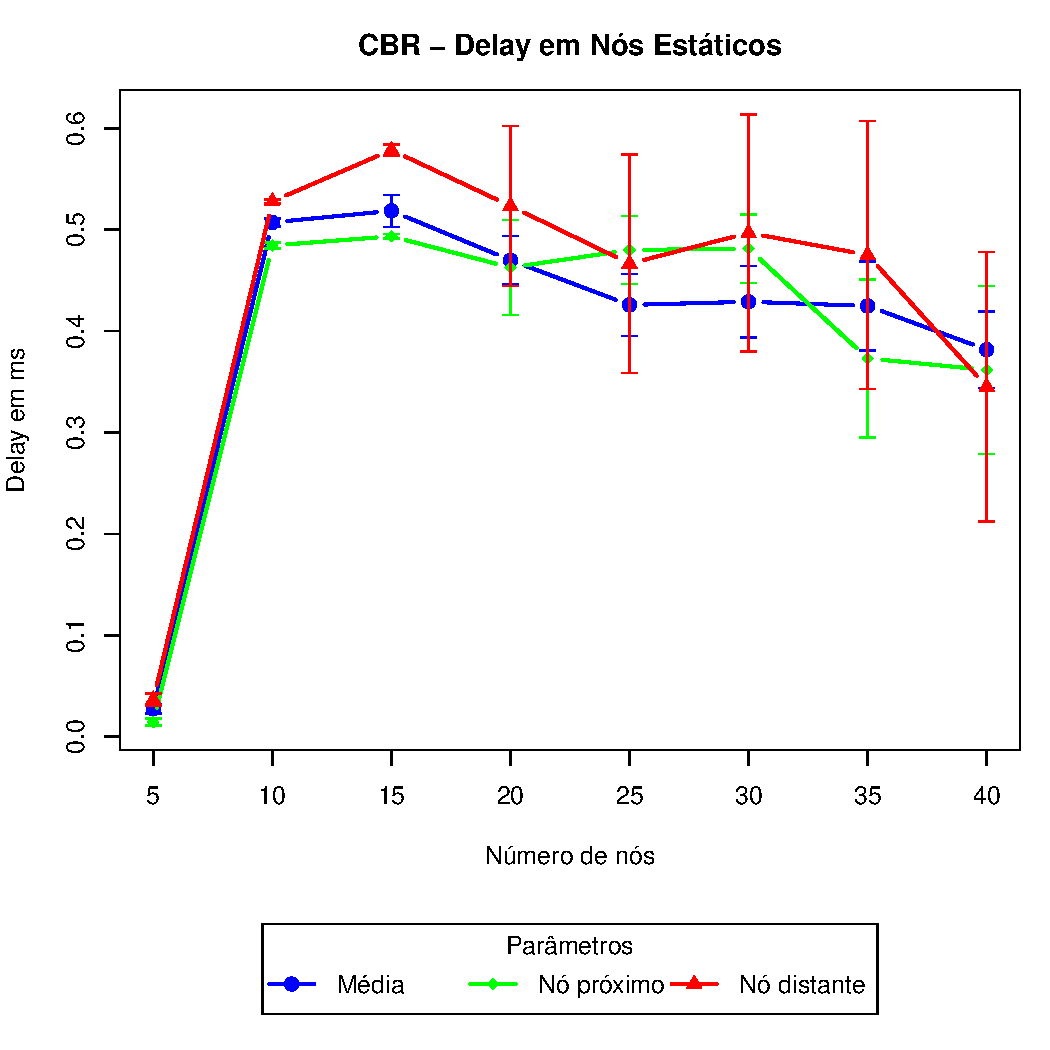
\includegraphics[width=.7\textwidth]{images/DelayPackets_static_CBR.pdf}}%
%}
%\end{center}
%\caption{Tempo médio de atraso na entrega de pacotes a partir de nós sem mobilidade utilizando tráfego de dados constante (CBR/UDP).}
%\label{fig:delayPackets_static_CBR}
%\end{figure}


\subsection{Perda de pacotes}\label{subsec:perda}

A segunda métrica utilizada para avaliar o comportamento da rede é através da perda de pacotes. A perda de pacotes apresentadas durante todo o tempo de execução da simulação, 60 segundos, são exibidas para cada um dos quatro cenários abordados, variando o modelo de tráfego (CBR e rajada) e a adoção ou não de mobilidade por parte dos dispositivos.

A Figura \ref{fig:lostPackets_static} apresenta os resultados para os cenários que não consideram a mobilidade dos dispositivos. Nesse contexto foram comparados os cenários em que se utilizam os modelos de tráfego em rajada e CBR. Para cada cenário foram computadas as perdas de pacotes referentes à média de toda a rede, aos dispositivos localizados mais próximos ao ponto de acesso e aos dispositivos mais distantes ao ponto de acesso.

As redes que adotaram o tráfego constante de dados apresentaram em média, um volume maior de pacotes perdidos se comparadas com as redes que adotaram o tráfego em rajada.

\begin{figure}[H]
\begin{center}
{%
\setlength{\fboxsep}{2pt}%
\setlength{\fboxrule}{1pt}%
\fbox{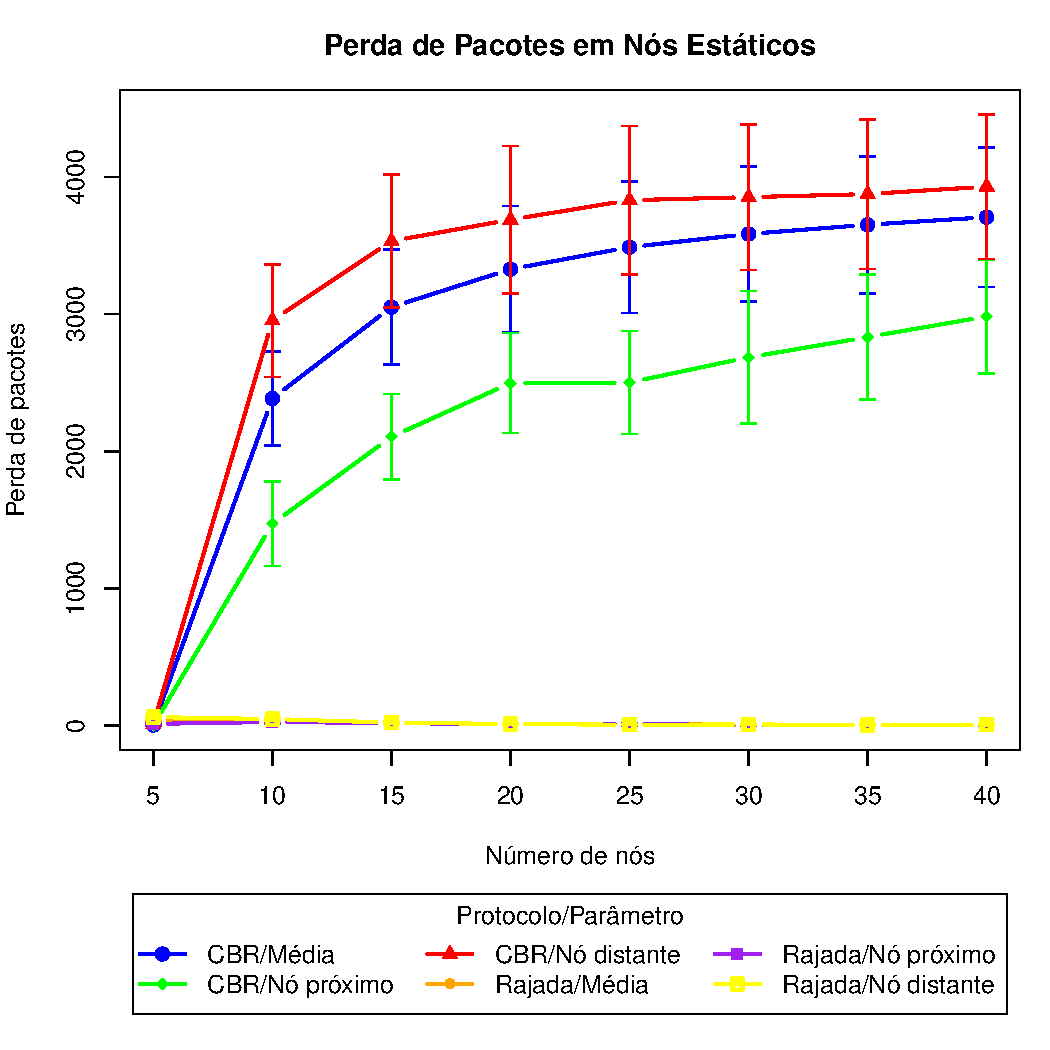
\includegraphics[width=.7\textwidth]{images/LostPackets_static.pdf}}%
}
\end{center}
\caption{Taxa de perda de pacotes em nós estáticos considerando os modelos de tráfego em rajada e CBR.}
\label{fig:lostPackets_static}
\end{figure}

As redes que utilizaram o tráfego CBR apresentaram um crescimento no número de pacotes perdidos de acordo com o aumento no número de dispositivos na rede. Este comportamento é justificado pelo fato de que com o aumento no número de dispositivos, mais pacotes serão transmitidos na rede e assim, proporcionalmente também aumentarão o número de colisões, gerando maiores perdas de pacotes. Como o protocolo utilizado nesse cenário é o UDP, não há nenhum mecanismo por parte do protocolo para diminuir no número de colisões.

Os dispositivos localizados próximo ao ponto de acesso apresentaram uma menor volume de pacotes perdidos em comparação à média, ao contrário do que ocorre com os dispositivos distantes do AP, que apresentaram uma maior perda. Este comportamento é esperado visto que os nós próximos enfrentam um meio um pouco menos congestionado até o ponto de acesso, já os dispositivos distantes enfrentam uma maior probabilidade de colisão com os pacotes dos demais dispositivos da rede.

As redes que utilizaram tráfego em rajada não apresentaram um aumento significativo no número de pacotes perdidos durante a simulação, resultados justificados pelo uso do protocolo TCP nesse cenário. Ao se detectar um aumento no número de colisões devido ao aumento no número de dispositivos atuantes na rede, o protocolo TCP aumenta a janela de congestionamento, diminuindo a vazão do link, como visto na Figura \ref{fig:throughput_CBR_pulse}, e assim mantendo a taxa de perda de pacotes estável.

Como apresentado na Figura \ref{fig:lostPackets_CBR_pulse}, a incorporação de um modelo para mobilidade dos dispositivos, utilizando os parâmetros descritos na Seção \ref{sec:proj_e_criterios}, não trouxe alterações significativas no desempenho médio dos modelo tráfego.

\begin{figure}[H]
\begin{center}
{%
\setlength{\fboxsep}{2pt}%
\setlength{\fboxrule}{1pt}%
\fbox{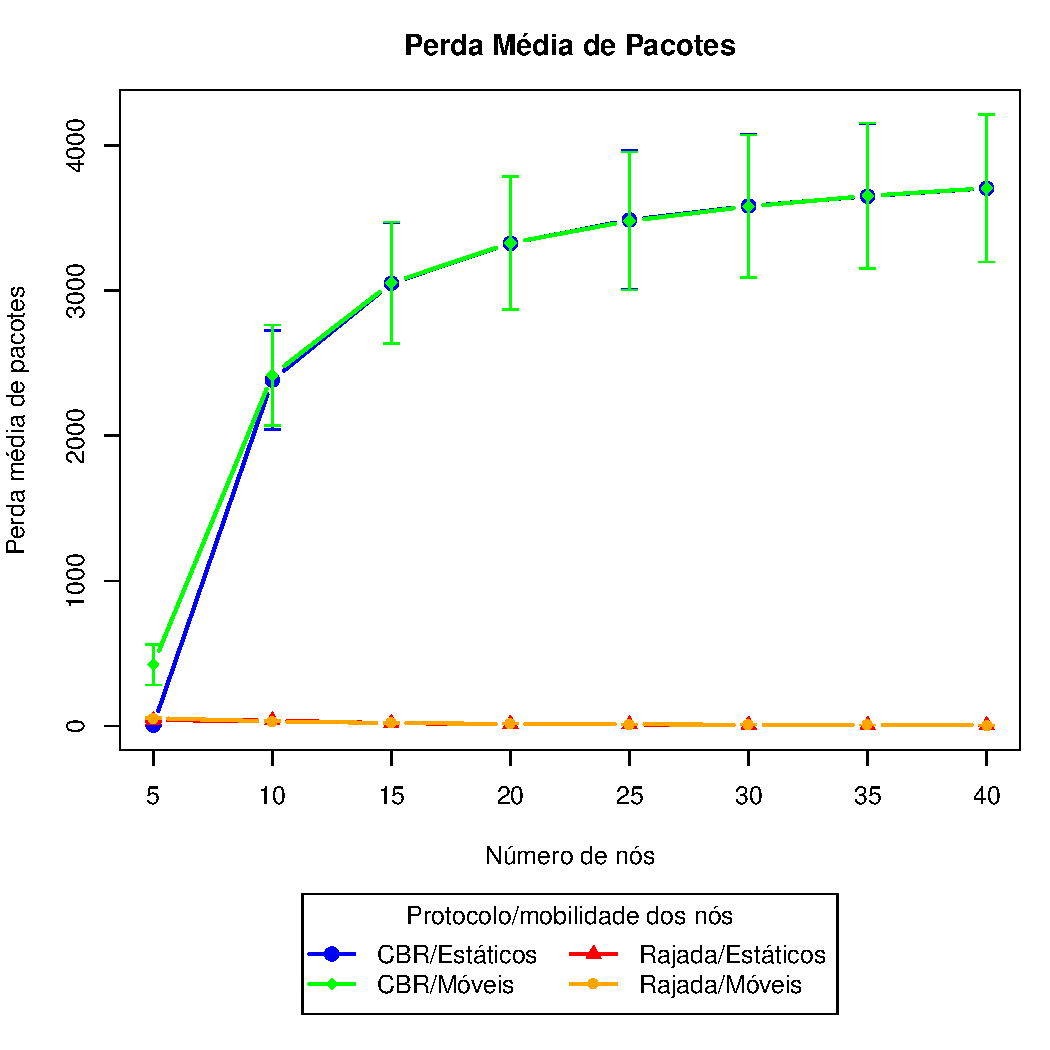
\includegraphics[width=.7\textwidth]{images/LostPackets_CBR_pulse.pdf}}%
}
\end{center}
\caption{Taxa média de perda de pacotes em cada cenário durante a execução da simulação.}
\label{fig:lostPackets_CBR_pulse}
\end{figure}

%\begin{figure}[H]
%\begin{center}
%{%
%\setlength{\fboxsep}{2pt}%
%\setlength{\fboxrule}{1pt}%
%\fbox{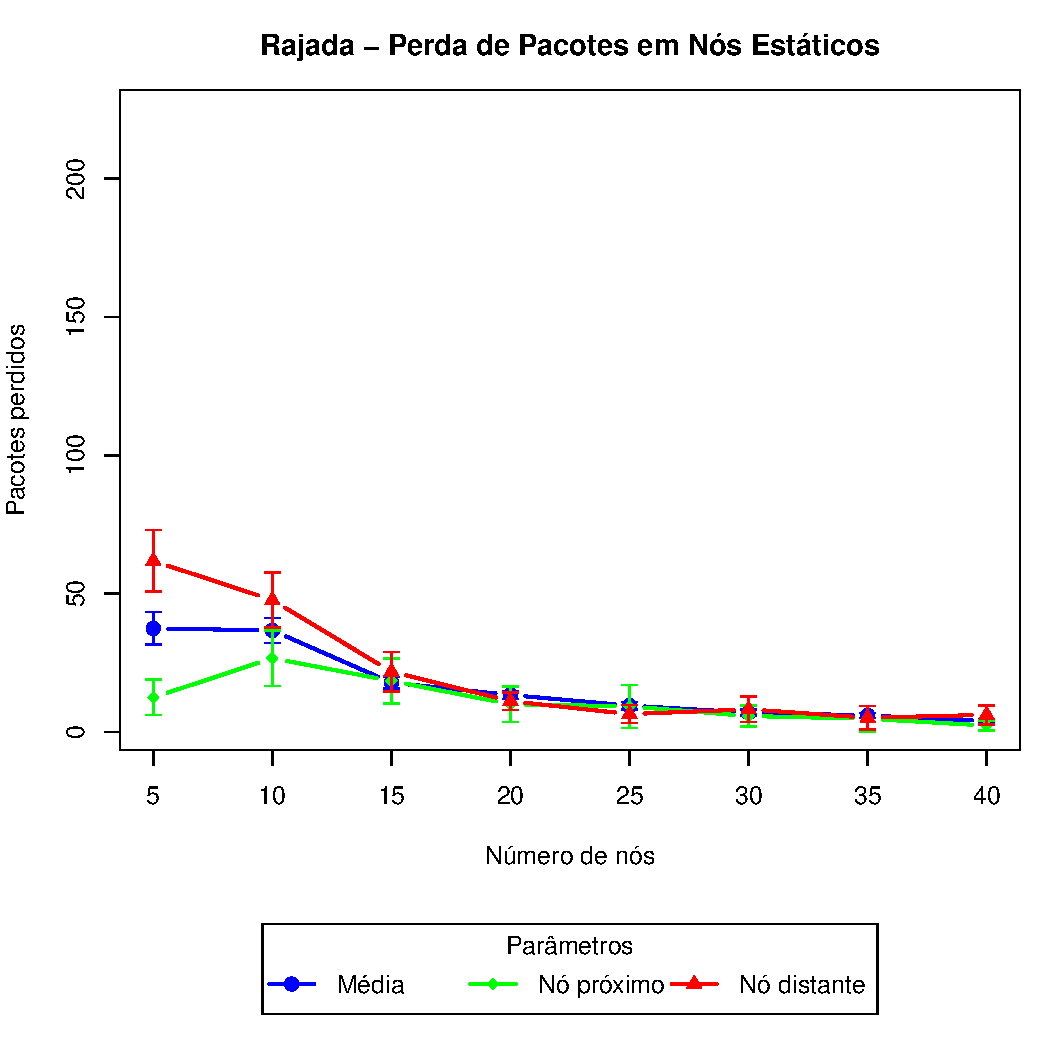
\includegraphics[width=.7\textwidth]{images/LostPackets_static_pulse.pdf}}%
%}
%\end{center}
%\caption{VOID}
%\label{fig:lostPackets_static_pulse}
%\end{figure}

%\begin{figure}[H]
%\begin{center}
%{%
%\setlength{\fboxsep}{2pt}%
%\setlength{\fboxrule}{1pt}%
%\fbox{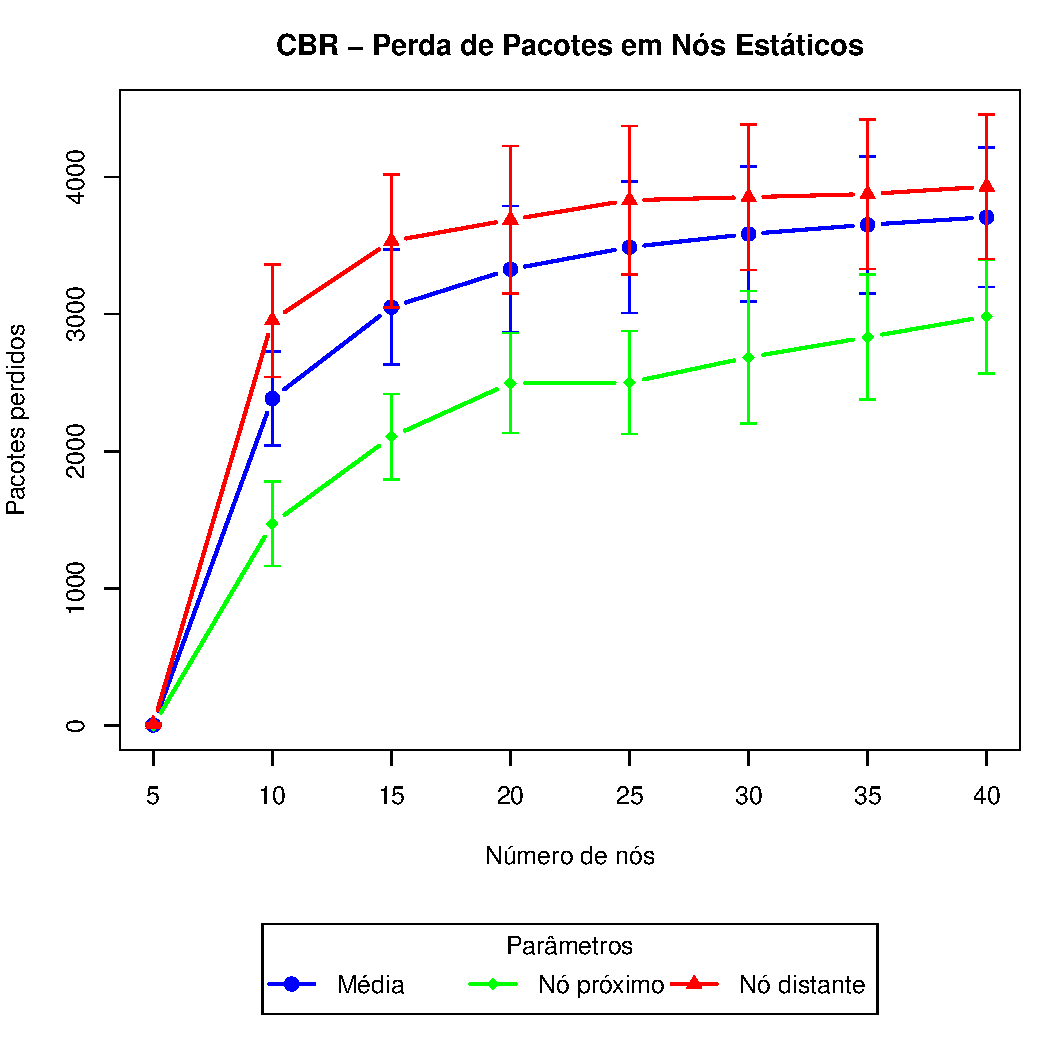
\includegraphics[width=.7\textwidth]{images/LostPackets_static_CBR.pdf}}%
%}
%\end{center}
%\caption{VOID}
%\label{fig:lostPackets_static_CBR}
%\end{figure}

\subsection{Vazão}\label{subsec:vazao}

A taxa de transferência ou \textit{throughput}, é outra métrica adotada para avaliar o desempenho da rede nos cenários considerados. Para todos os cenários foi determinado que a taxa de dados limite da rede sem fio fosse 512 Kbps e o link do AP até o servidor fosse de 5 Mbps.

A Figura~\ref{fig:throughput_static} apresenta as taxas de transferências para redes compostas por nós estáticos. Os dispositivos que utilizam o CBR confirmaram taxa constante de transferência, independente do número de dispositivos que compõem a rede. Dado que essa abordagem utiliza o protocolo UDP para realizar as transmissões, independente do número de colisões que a conexão possa sofrer devido ao crescimento da rede, como visto na Figura \ref{fig:lostPackets_static}, a taxa de transmissão continua constante.

Os dispositivos que realizam o tráfego em rajada apresentaram uma queda na vazão a medida que mais dispositivos eram adicionados à rede. Devido a utilização do protocolo TCP, para não aumentar o volume de pacotes perdidos durante a transferência, o protocolo decide aumentar a janela de colisão, o que acarreta em uma maior espera para realizar a transmissão de pacotes e assim, diminuindo a vazão da rede.

Dispositivos próximos ao ponto de acesso apresentaram uma maior taxa de transferência comparados à média, diferentemente dos dispositivos distantes, que apresentaram um desempenho um pouco inferior à média.

\begin{figure}[H]
\begin{center}
{%
\setlength{\fboxsep}{2pt}%
\setlength{\fboxrule}{1pt}%
\fbox{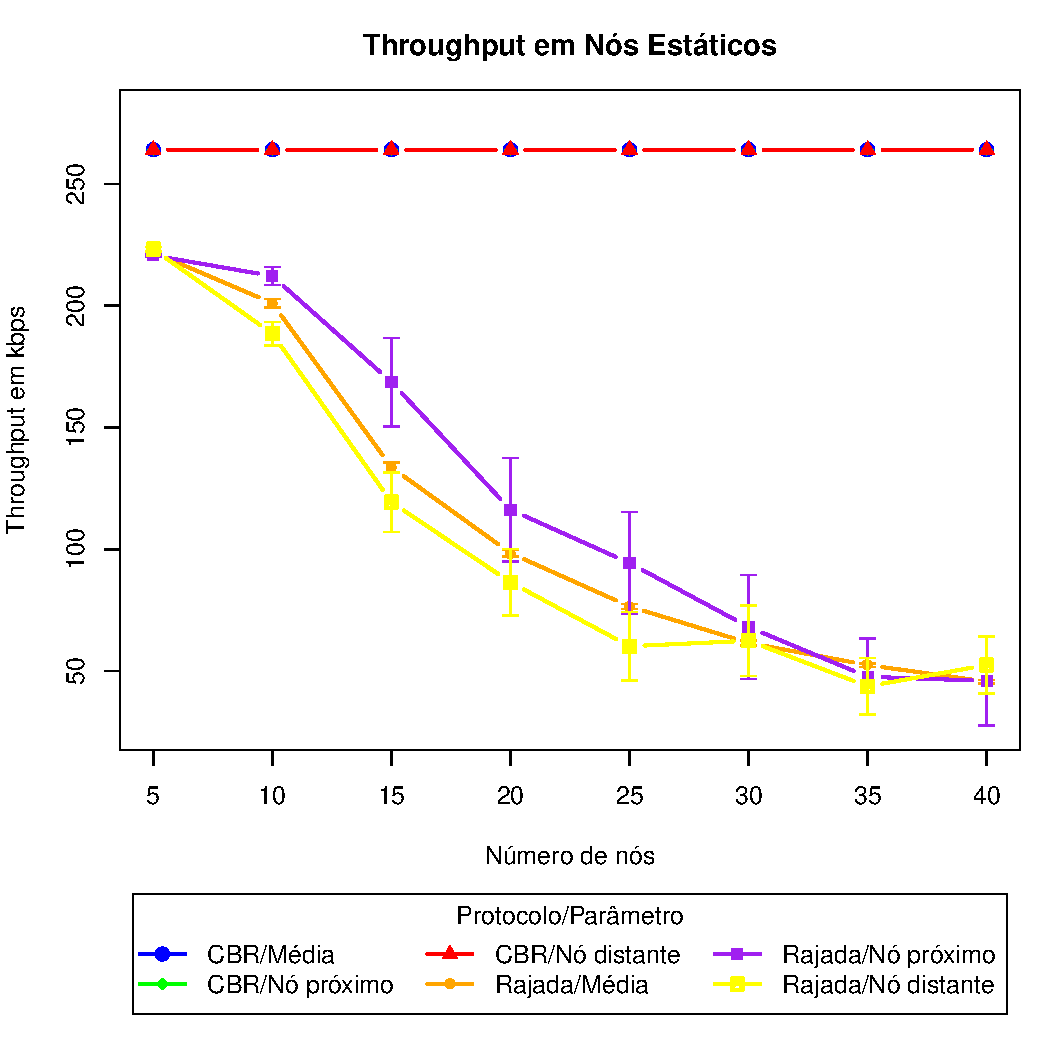
\includegraphics[width=.7\textwidth]{images/Throughput_static.pdf}}%
}
\end{center}
\caption{\textit{Throughput} médio na comunicação de dispositivos estáticos com o AP em comparação com os resultados do dispositivo mais próximo e o mais distante do AP, considerando os modelos de tráfego em rajada e CBR.}
\label{fig:throughput_static}
\end{figure}
 
Ao se considerar um cenário composto por dispositivos móveis, ao realizar o tráfego em rajada, nós com mobilidade apresentaram, em média, uma vazão significativamente inferior aos nós estáticos. Para nós que utilizam CBR, como esperado, não houve mudanças significativas de desempenho. A Figura \ref{fig:throughput_CBR_pulse} apresenta os resultados para esses cenários. 

\begin{figure}[H]
\begin{center}
{%
\setlength{\fboxsep}{2pt}%
\setlength{\fboxrule}{1pt}%
\fbox{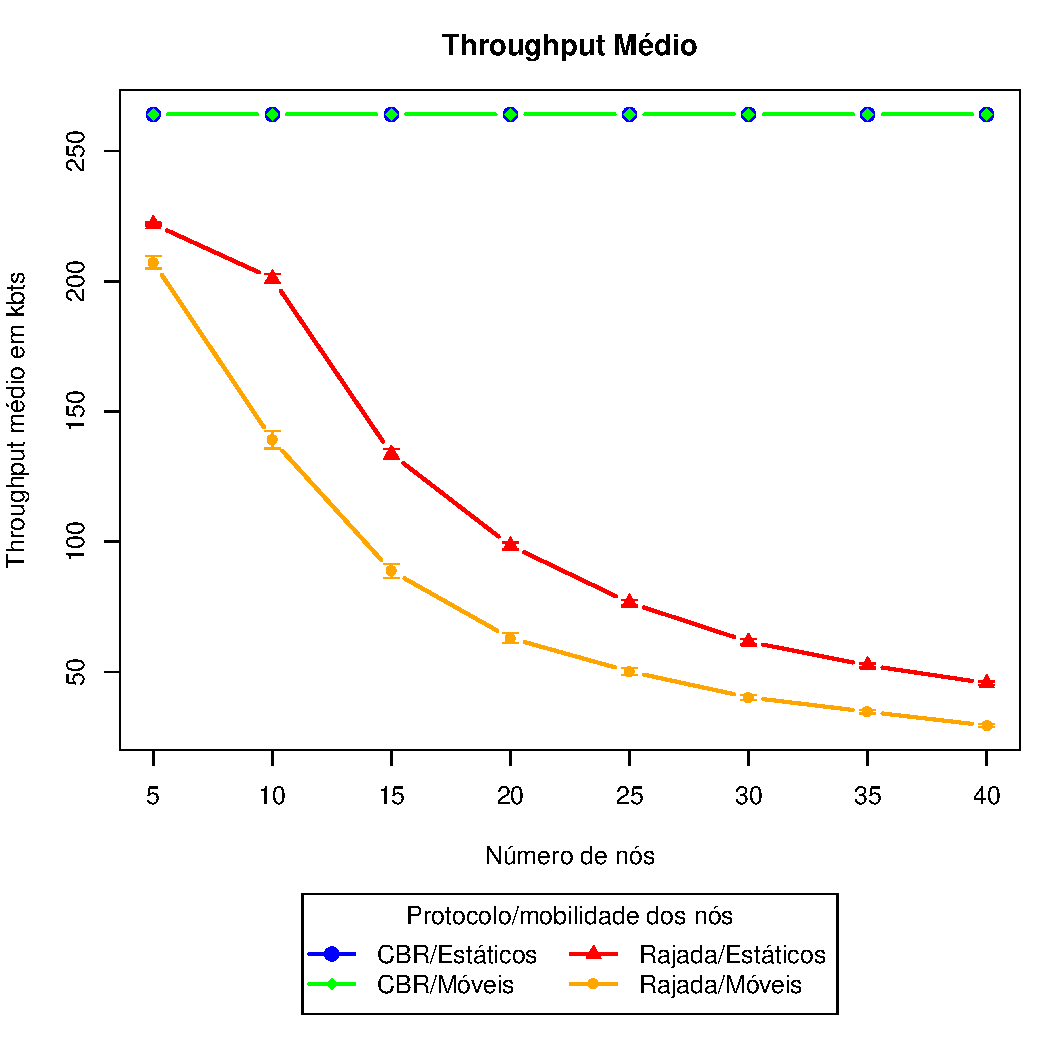
\includegraphics[width=.7\textwidth]{images/Throughput_CBR_pulse.pdf}}%
}
\end{center}
\caption{\textit{Throughput} médio dos dispositivos considerando os modelos de tráfego em rajada e CBR e nós estáticos e móveis.}
\label{fig:throughput_CBR_pulse}
\end{figure}

%\begin{figure}[H]
%\begin{center}
%{%
%\setlength{\fboxsep}{2pt}%
%\setlength{\fboxrule}{1pt}%
%\fbox{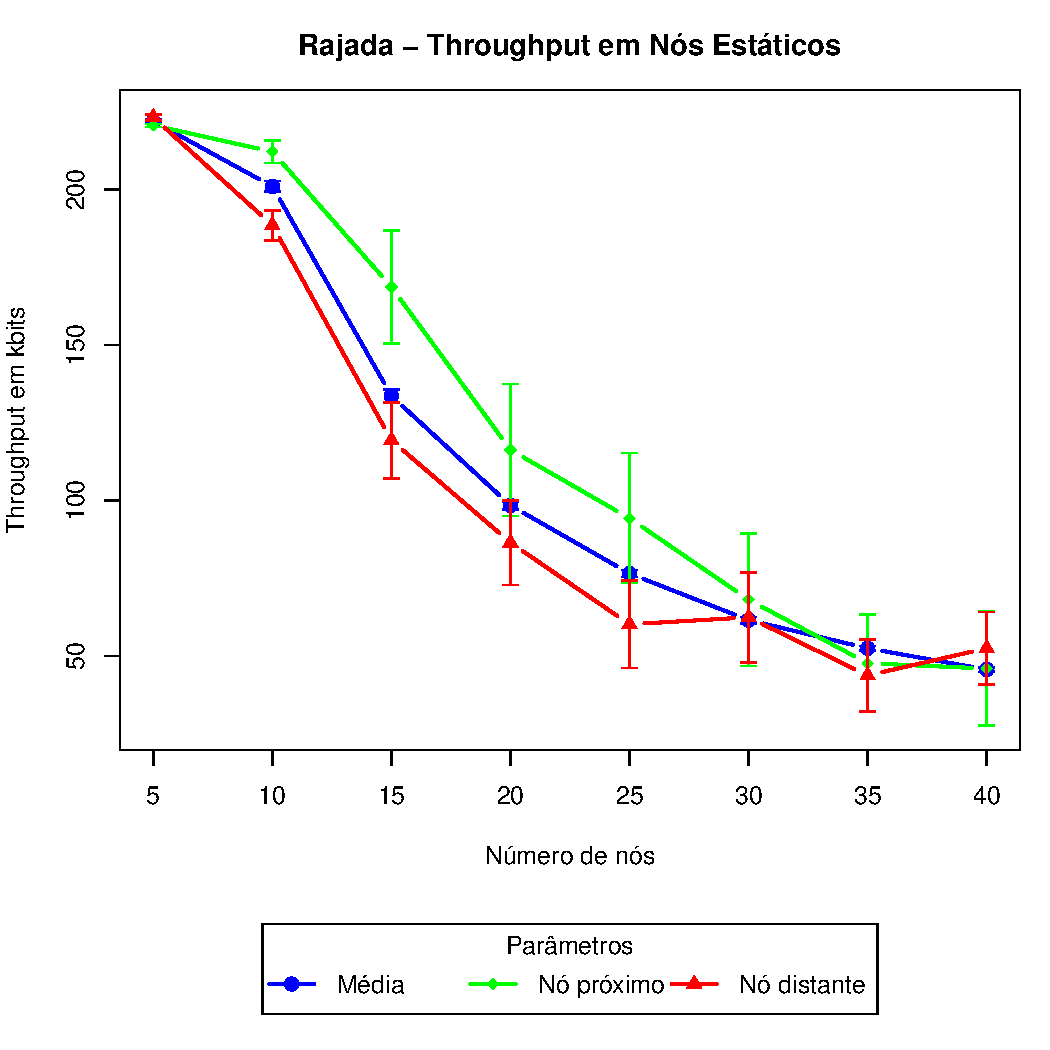
\includegraphics[width=.7\textwidth]{images/Throughput_static_pulse.pdf}}%
%}
%\end{center}
%\caption{VOID}
%\label{fig:throughput_static_pulse}
%\end{figure}

\section{Conclusões}

A partir dos resultados apresentados na Seção \ref{sec::resultados} pode-se obter algumas conclusões a respeito do desempenho da rede utilizando as métricas de vazão, perda de pacotes e atraso na entrega de pacotes.

A respeito do tempo de atraso na entrega de pacotes, os dispositivos que utilizaram CBR como modelo de transmissão de dados apresentaram um maior tempo de atraso comparados com os dispositivos que realizaram tráfego em rajada. Ao considerar um modelo de mobilidade dos dispositivos nesse cenário, os nós móveis apresentaram um atraso um pouco superior comparados com os cenários equivalentes utilizando nós estáticos.

Com relação à perda de pacotes, redes compostas por dispositivos utilizando CBR, a perda de pacotes se mostrou muito superior às taxas apresentadas pelos dispositivos realizando tráfego em rajada. A medida em que a rede aumenta, o número de colisões tende a crescer. Dado que o tráfego em rajada está utilizando o protocolo TCP para realizar as transmissões, o protocolo ao detectar um aumento no número de colisões, aumenta a janela de colisões para evitar a ocorrência das mesmas, porém, com isso, diminui a vazão da rede. O protocolo UDP, utilizado com o tráfego CBR, não faz uso desse mecanismo, enviando sempre o máximo de dados possível porém, se sujeitando ao aumento no número de colisões. Para a métrica de perda de pacotes, cenários que consideravam a mobilidade dos dispositivos não apresentaram resultados significativamente diferentes dos cenários com nós estáticos.

A vazão da rede também foi avaliada. Redes que realizaram tráfego em rajada apresentaram uma queda considerável na vazão da rede a medida que mais nós eram adicionados. Esse comportamento ocorreu devido ao protocolo utilizado, o TCP, que, como mencionado anteriormente, ao detectar um aumento no número de colisões, realiza procedimentos para evitá-las, porém como efeito colateral acaba diminuindo a vazão da rede. Dispositivos próximos ao ponto de acesso apresentaram uma vazão significativa superior à média nesse cenário e, como esperado, dispositivos distantes apresentaram um desempenho inferior à média.

Redes que utilizaram CBR apresentaram uma vazão fixa para todos os nós, independentemente do número de dispositivos compondo a rede. Como esperado, devido a utilização do protocolo UDP que, diferentemente do TCP, não realiza nenhum mecanismo para tratar colisões na rede. Independe se há colisões na transmissão, o protocolo UDP envia todos os pacotes que o meio de transmissão lhe permite, refletindo na vazão constante apresentada nos resultados.

Ao comparar os resultados das redes com nós estáticos com redes permitindo a mobilidade dos dispositivos, nota-se um desempenho inferior dos nós móveis quando realizam  trafego em rajada.

Analisando simultaneamente os resultados apresentados pelas três métricas, pode-se destacar a coerência entre as curvas referentes à vazão e à perda de pacotes. Em dispositivos realizando tráfego em rajada, à medida em que o número de dispositivos aumenta, a vazão diminui como resposta as medidas executas para manter o nível de perda de pacotes estável. Para nós utilizando CBR, mantendo a vazão constante, o número de pacotes perdidos cresce significativamente.

\bibliographystyle{config/sbc}
\bibliography{sbc-template}

\end{document}